\documentclass{beamer}
\usetheme{default}
\beamertemplatenavigationsymbolsempty
\usepackage{rembeamer}
\usepgfplotslibrary{statistics} 

\begin{document}

\begin{frame}
  \begin{itemize}
    \item[] Using measures of central tendency and spread to describe
    data. 
  \end{itemize}
\end{frame}

\begin{frame}
  \frametitle{Loans Data - Mean or Average}
  \centering
  \begin{tikzpicture}
    \begin{axis}[
      xmin=5,
      xmax=25,
      xlabel={Interest Rate (Percentage)},
      ylabel={Count}
    ]
      \addplot+ [
        hist={bins=8},
        fill=orange,
        draw=black,
        mark=none
      ]
      table [y=interest_rate,col sep=tab] {../data/loans50.dat};
    \end{axis}
  \end{tikzpicture}
\end{frame}

\begin{frame}
  \frametitle{Mean or Average}
  \begin{displaymath}
    \begin{array}{rcl}
      \text{Numeric Variable} & = & \{x_1, x_2, \ldots, x_n \} \\[2em]
      \bar{x} & = & \frac{x_1 + x_2 + \ldots + x_n}{n} \\[2em]
      \text{Loans Data } \bar{x} & = & 11.57 
    \end{array}
  \end{displaymath} 
\end{frame}

\begin{frame}
  \frametitle{Loans Data - Deviation and Variance}
  \centering
  \begin{tikzpicture}
    \begin{axis}[
      xmin=5,
      xmax=25,
      xlabel={Interest Rate (Percentage)},
      ylabel={Count}
    ]
      \addplot+ [
        hist={bins=8},
        fill=orange,
        draw=black,
        mark=none
      ]
      table [y=interest_rate,col sep=tab] {../data/loans50.dat};
    \end{axis}
  \end{tikzpicture}
\end{frame}

\begin{frame}
  \frametitle{Deviations}
  \begin{displaymath}
    \begin{array}{rcl}
      x_1 - \bar{x} & = & 10.9 - 11.57 = -0.67 \\[0.3em]
      x_2 - \bar{x} & = & 9.92 - 11.57 = -1.65 \\[0.3em]
      x_3 - \bar{x} & = & 26.3 - 11.57 = 14.73 \\[0.3em]
      & \vdots & \\[0.3em]
      x_{50} - \bar{x} & = & 6.08 - 11.57 = -5.49 
    \end{array}
  \end{displaymath} 
\end{frame}

\begin{frame}
  \frametitle{Sample Variance}
  \begin{displaymath}
    \begin{array}{rcl}
      x_1 - \bar{x} & = & 10.9 - 11.57 = -0.67 \\[0.3em]
      x_2 - \bar{x} & = & 9.92 - 11.57 = -1.65 \\[0.3em]
      x_3 - \bar{x} & = & 26.3 - 11.57 = 14.73 \\[0.3em]
      & \vdots & \\[0.3em]
      x_{50} - \bar{x} & = & 6.08 - 11.57 = -5.49 \\[1em]
      s^2 & = & \frac{(-0.67)^2 + (-1.65)^2 + (14.73)^2 + \ldots +
      (-5.49)^2}{50-1} \\[1em]
      & = & \frac{0.45 + 2.72 + \ldots + 30.14}{49} = 25.52 
    \end{array}
  \end{displaymath} 
\end{frame}

\begin{frame}
  \frametitle{Standard Deviation}
  \begin{displaymath}
    \begin{array}{rcl}
      x_1 - \bar{x} & = & 10.9 - 11.57 = -0.67 \\[0.3em]
      x_2 - \bar{x} & = & 9.92 - 11.57 = -1.65 \\[0.3em]
      x_3 - \bar{x} & = & 26.3 - 11.57 = 14.73 \\[0.3em]
      & \vdots & \\[0.3em]
      x_{50} - \bar{x} & = & 6.08 - 11.57 = -5.49 \\[1em]
      s^2 & = & \frac{(-0.67)^2 + (-1.65)^2 + (14.73)^2 + \ldots +
      (-5.49)^2}{50-1} \\[1em]
      & = & \frac{0.45 + 2.72 + \ldots + 30.14}{49} = 25.52 \\[1em]
      s & = & \sqrt{25.52} = 5.05 
    \end{array}
  \end{displaymath} 
\end{frame}

\begin{frame}
  \frametitle{Loans Data - Standard Deviation}
  \centering
  \begin{tikzpicture}
    \begin{axis}[
      xmin=5,
      xmax=25,
      xlabel={Interest Rate (Percentage)},
      ylabel={Count}
    ]
      \addplot+ [
        hist={bins=8},
        fill=orange,
        draw=black,
        mark=none
      ]
      table [y=interest_rate,col sep=tab] {../data/loans50.dat};
    \end{axis}
  \end{tikzpicture}
\end{frame}

\begin{frame}
  \frametitle{Loans - Median}
  \begin{table}
    \begin{tabular}{@{}cccccccc@{}}
      \toprule
      5.31 & 5.31 & 5.32 & 6.08 & 6.08 & 6.08 & 6.71 & 6.71 
      \\[0.3em]
      7.34 & 7.34 & 7.35 & 7.96 & 7.96 & 7.96 & 7.97 & 9.43 
      \\[0.3em]
      9.43 & 9.44 & 9.44 & 9.44 & 9.92 & 9.92 & 9.92 & 9.92 
      \\[0.3em]
      9.93 & 9.93 & 10.42 & 10.42 & 10.90 & 10.90 & 10.91 & 10.91 
      \\[0.3em]
      10.91 & 11.98 & 12.62 & 12.62 & 12.62 & 14.08 & 15.04 & 16.02
      \\[0.3em]
      17.09 & 17.09 & 17.09 & 18.06 & 18.45 & 19.42 & 20.00 & 21.45
      \\[0.3em]
      24.85 & 26.30 \\
      \bottomrule 
    \end{tabular}
  \end{table}
  \begin{equation*}
    M = 9.93 
  \end{equation*}
\end{frame}

\begin{frame}
  \frametitle{Loans - Percentile and Quartiles}
  \begin{table}
    \begin{tabular}{@{}cccccccc@{}}
      \toprule
      5.31 & 5.31 & 5.32 & 6.08 & 6.08 & 6.08 & 6.71 & 6.71 
      \\[0.3em]
      7.34 & 7.34 & 7.35 & 7.96 & 7.96 & 7.96 & 7.97 & 9.43 
      \\[0.3em]
      9.43 & 9.44 & 9.44 & 9.44 & 9.92 & 9.92 & 9.92 & 9.92 
      \\[0.3em]
      9.93 & 9.93 & 10.42 & 10.42 & 10.90 & 10.90 & 10.91 & 10.91 
      \\[0.3em]
      10.91 & 11.98 & 12.62 & 12.62 & 12.62 & 14.08 & 15.04 & 16.02
      \\[0.3em]
      17.09 & 17.09 & 17.09 & 18.06 & 18.45 & 19.42 & 20.00 & 21.45
      \\[0.3em]
      24.85 & 26.30 \\
      \bottomrule 
    \end{tabular}
  \end{table}
  \begin{equation*}
    M = 9.93 \hspace{0.7cm}
    Q_1 = 7.96 \hspace{0.7cm}
    Q_3 = 14.08 
  \end{equation*}
\end{frame}

\begin{frame}
  \frametitle{Loans - Interquartile Range and Outliers}
  \begin{table}
    \begin{tabular}{@{}cccccccc@{}}
      \toprule
      5.31 & 5.31 & 5.32 & 6.08 & 6.08 & 6.08 & 6.71 & 6.71 
      \\[0.3em]
      7.34 & 7.34 & 7.35 & 7.96 & 7.96 & 7.96 & 7.97 & 9.43 
      \\[0.3em]
      9.43 & 9.44 & 9.44 & 9.44 & 9.92 & 9.92 & 9.92 & 9.92 
      \\[0.3em]
      9.93 & 9.93 & 10.42 & 10.42 & 10.90 & 10.90 & 10.91 & 10.91 
      \\[0.3em]
      10.91 & 11.98 & 12.62 & 12.62 & 12.62 & 14.08 & 15.04 & 16.02
      \\[0.3em]
      17.09 & 17.09 & 17.09 & 18.06 & 18.45 & 19.42 & 20.00 & 21.45
      \\[0.3em]
      24.85 & 26.30 \\
      \bottomrule 
    \end{tabular}
  \end{table}
  \begin{equation*}
    M = 9.93 \hspace{0.7cm}
    Q_1 = 7.96 \hspace{0.7cm}
    Q_3 = 14.08
  \end{equation*}
  \begin{equation*}
    IQR = Q_3 - Q_1 = 14.08 - 7.96 = 6.12
  \end{equation*}
  \begin{equation*}
    (1.5) IQR = 9.18 \hspace{0.4cm}
    Q_3 + (1.5) IQR = 14.08 + 9.18 = 23.26
  \end{equation*}
\end{frame}

\begin{frame}
  \frametitle{Box Plot - Loans}
  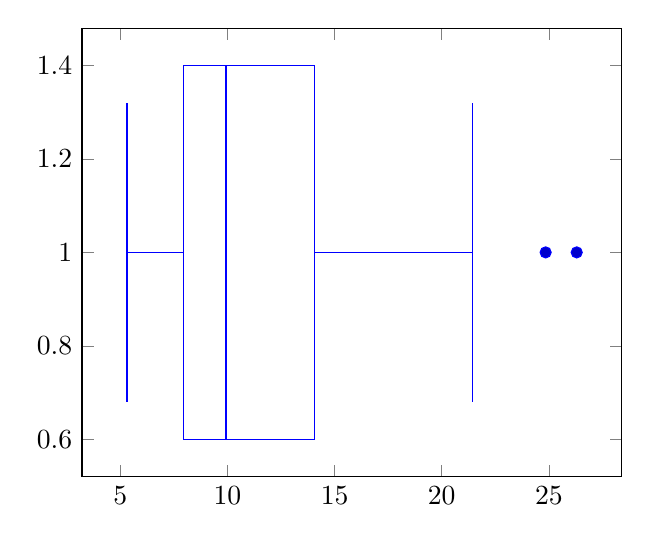
\begin{tikzpicture}
    \begin{axis}
      \addplot+ [
        boxplot prepared={
            lower whisker=5.31,
            lower quartile=7.96,
            median=9.93,
            upper quartile=14.08,
            upper whisker=21.45,
        },
      ] table [row sep=\\,y index=0] {
          data\\ 24.85 \\ 26.30 \\
      };
    \end{axis}
  \end{tikzpicture}
\end{frame}

\end{document}
